\documentclass[aspectratio=169]{beamer}
\usetheme{Madrid}
\usecolortheme{default}
\usepackage[T1]{fontenc}
\usepackage[utf8]{inputenc}
\usepackage{graphicx}
\usepackage{booktabs}
\usepackage{hyperref}

\title{Air Quality Intelligence System}
\subtitle{Advanced Database Management Systems}
\author{Péter Dobosi (MW79ON)}
\institute{University of Pannonia}
\date{2025/26 Spring}

\begin{document}

% ----------------------------------------------------------
\begin{frame}
\titlepage
\end{frame}

% ----------------------------------------------------------
\begin{frame}{Problem Statement}
\begin{itemize}
  \item Urban air pollution is a growing health concern
  \item Publicly available sensor data (OpenAQ) lacks real-time alerting
  \item Need: automated ingestion, threshold-based alerting, and operational oversight
\end{itemize}
\vspace{1em}
\textbf{Goal:} Build a production-ready DBMS-backed monitoring system demonstrating:\\
triggers, transactions, partitioning, indexing, backups, and an operational GUI.
\note{~1 min --- set the scene, explain why this matters.}
\end{frame}

% ----------------------------------------------------------
\begin{frame}{Architecture Overview}
\begin{figure}
\centering
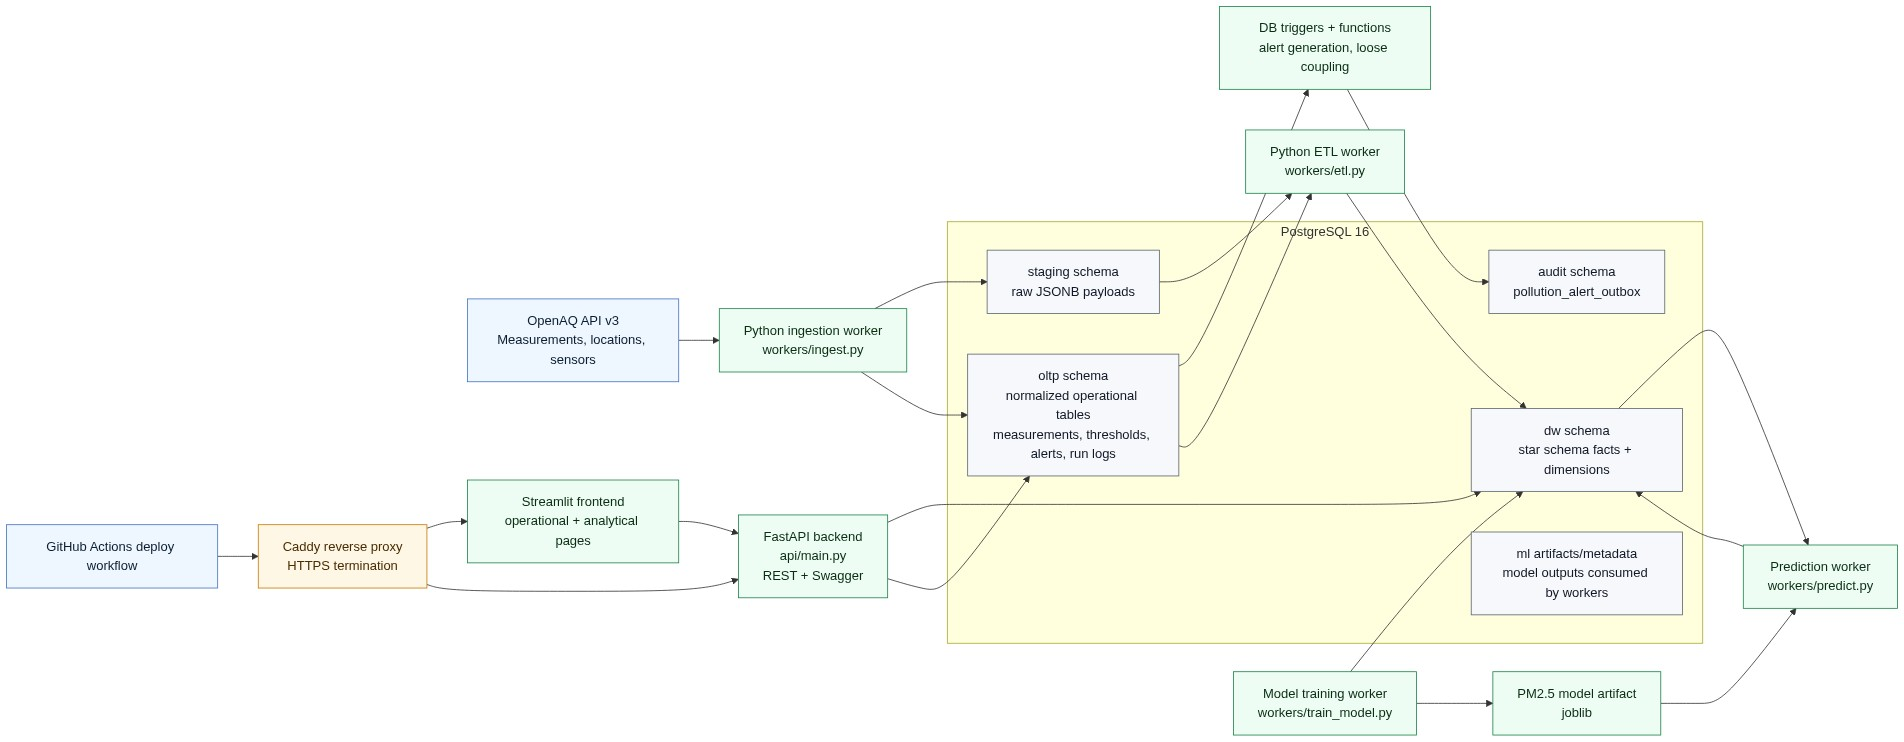
\includegraphics[width=0.72\textwidth]{../../diagrams/system_architecture.png}
\end{figure}
\note{~1 min --- walk through the components left-to-right.}
\end{frame}

% ----------------------------------------------------------
\begin{frame}{Technologies Used}
\begin{columns}[T]
\begin{column}{0.5\textwidth}
\begin{itemize}
  \item PostgreSQL 16
  \item PL/pgSQL triggers
  \item Range partitioning
  \item Explicit transactions
  \item CHECK / FK constraints
\end{itemize}
\end{column}
\begin{column}{0.5\textwidth}
\begin{itemize}
  \item Python 3.12
  \item FastAPI (REST)
  \item Streamlit (GUI)
  \item Docker Compose
  \item Caddy (HTTPS)
  \item GitHub Actions (CI/CD)
\end{itemize}
\end{column}
\end{columns}
\note{~1 min --- highlight the PostgreSQL-specific features.}
\end{frame}

% ----------------------------------------------------------
\begin{frame}{Demo: Operational GUI --- Stations \& Measurements}
\begin{itemize}
  \item Station Explorer page: select city → station → parameter
  \item Shows time-series chart and raw measurement table
  \item Data comes from \texttt{oltp.measurement\_raw} (partitioned)
\end{itemize}
\vspace{0.5em}
\textit{Live demo: open \url{https://mw79on-demo.online}, navigate to Station Explorer}
\note{~1.5 min --- show the live dashboard.}
\end{frame}

% ----------------------------------------------------------
\begin{frame}{Demo: Threshold Management}
\begin{itemize}
  \item CRUD interface for \texttt{oltp.threshold\_rule}
  \item Each rule: city + pollutant + severity level + minimum value
  \item Unique constraint: \texttt{(parameter\_id, city, warning\_level)}
\end{itemize}
\vspace{0.5em}
\textit{Live demo: add/edit a threshold rule, show it persisted in the table.}
\note{~1.5 min --- create a rule, show constraint enforcement.}
\end{frame}

% ----------------------------------------------------------
\begin{frame}{Demo: Trigger-Based Alert Generation}
\begin{itemize}
  \item Trigger: \texttt{trg\_measurement\_generate\_pollution\_alert}
  \item Fires AFTER INSERT on \texttt{measurement\_raw}
  \item Matches value against active threshold rules → inserts alert row
  \item Second trigger enqueues event into \texttt{audit.pollution\_alert\_outbox}
\end{itemize}
\vspace{0.5em}
\textit{Live demo: insert measurement → observe new alert appearing.}
\note{~1.5 min --- explain trigger chain, show the alert table update.}
\end{frame}

% ----------------------------------------------------------
\begin{frame}{Demo: Alert Review \& Transaction Safety}
\begin{itemize}
  \item Alerts page: filter by status / severity
  \item Transition: open → reviewed → closed (with notes)
  \item Ingestion uses explicit transactions with savepoints
  \item Partial batch failure → atomic rollback, no corrupt data
\end{itemize}
\vspace{0.5em}
\textit{Live demo: review an alert; show ingestion log for transaction evidence.}
\note{~1.5 min --- review alert, point out transaction columns in logs.}
\end{frame}

% ----------------------------------------------------------
\begin{frame}{Demo: Indexing, Partitioning, Backup}
\begin{itemize}
  \item \texttt{measurement\_raw}: range-partitioned by month (25+ partitions)
  \item B-tree indexes on FKs and hot query columns
  \item \texttt{scripts/backup.sh}: \texttt{pg\_dump} with rotation \& optional off-site
  \item System Status page shows ingestion run history
\end{itemize}
\note{~1 min --- show partition list, index usage, backup script.}
\end{frame}

% ----------------------------------------------------------
\begin{frame}{Deployment \& DevOps}
\begin{columns}[T]
\begin{column}{0.55\textwidth}
\begin{itemize}
  \item Hetzner Cloud VM (Ubuntu 24.04)
  \item Docker Compose: 5 services
  \item Caddy: automatic HTTPS (Let's Encrypt)
  \item GitHub Actions: push → deploy
  \item Cron scheduling:
  \begin{itemize}
    \item Every 3h: ingest + ETL
    \item Daily: predictions
    \item Daily: backup with rotation
  \end{itemize}
\end{itemize}
\end{column}
\begin{column}{0.45\textwidth}
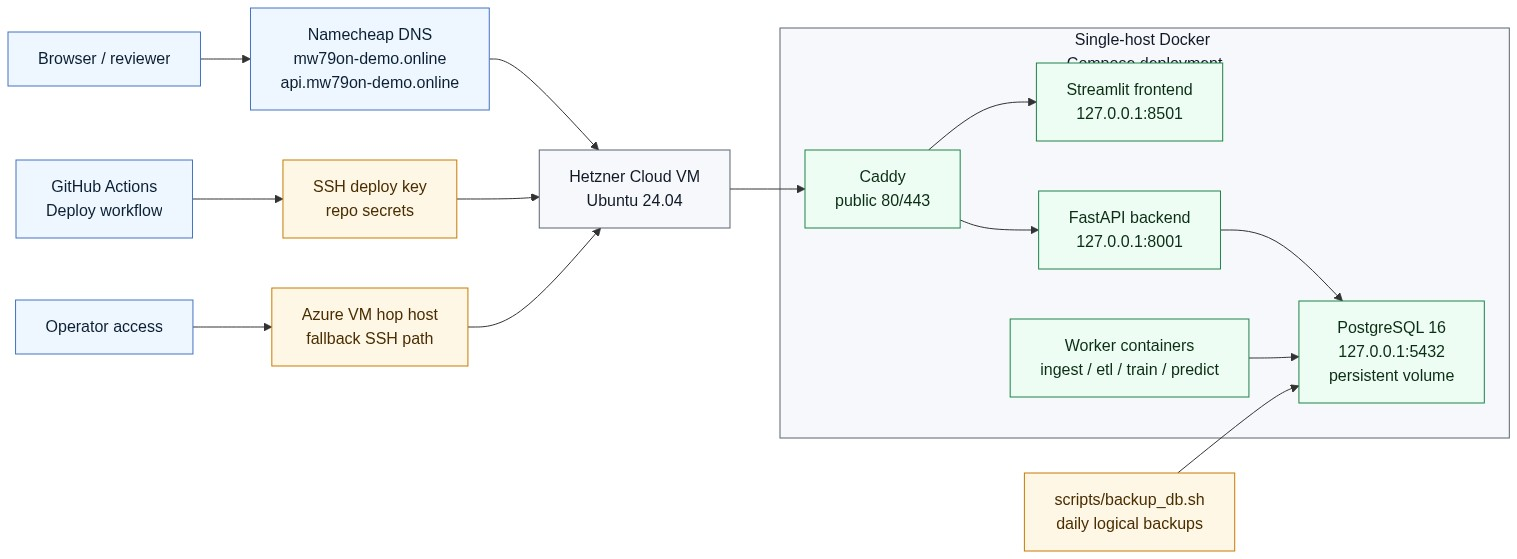
\includegraphics[width=\textwidth]{../../diagrams/deployment_architecture.png}
\end{column}
\end{columns}
\note{~1 min --- show workflow run in GitHub, live site.}
\end{frame}

% ----------------------------------------------------------
\begin{frame}{Summary \& Lessons Learned}
\begin{itemize}
  \item PostgreSQL triggers provide powerful event-driven logic
  \item Partitioning enables efficient time-range queries and archival
  \item Explicit transactions with savepoints ensure data integrity
  \item Docker Compose + Caddy = simple production deployment
  \item CI/CD keeps the system always up-to-date
\end{itemize}
\vspace{1em}
\textbf{Live system:} \url{https://mw79on-demo.online}\\
\textbf{Source code:} \url{https://github.com/dobosipeter/advanced-data-warehouse-and-database-management-systems-submission}
\note{~1 min --- wrap up, invite questions.}
\end{frame}

\end{document}
